\title{Simmulation Ideenverbreitung}
%TODO :
\subtitle{Praktikumsbericht}

\author{Arne Struck, Manuel Börries, Jonathan Werner}

\institute{Universität Hamburg \\ 
  Fakultät für Mathematik, Informatik und Naturwissenschaften \\
  Fachbereich Informatik, DKRZ \\
  Praktikum Paralleles Programmieren}
  
\date{\today}

\maketitle

\index{personen}{Struck, Arne}

\begin{abstract}
%TODO content
\quad \\
Aufgabenstellung: \\
Die Erstellung einer parallelen, clusterfähigen Simulation mittels MPI. \\ \\
Projekt Idee: \\
Die Untersuchung der Verbreitung von Meinungen, Vorstellungen innerhalb einer Population.
\keywords{Keywords}
\end{abstract}

\tableofcontents
\newpage
\section{Projekt-Idee}
Dieses Projekt soll die Verbreitung und Konkurrenz von Ideen im Sinne einer Weltanschauung, eines kontroversen Themas innerhalb einer begrenzten Population untersuchen und deren Mechanismen simulieren. Die Ideen sollen hierbei durch Kommunikation der Individuen und durch Entwicklung veränderbar sein. \\
Des weiteren darf es keine ''unrealistischen'' Entwicklungen geben. Niemand der gerade erst das Feuer entdeckt hat, baut am nächsten Tag eine Rakete, d.h. es gibt lediglich eine geringe Dichte qualtitativ hochwertiger Ideen.

\section{Modellierung} %von was?!
In diesem Abschnitt wird ein Überblick über die Modellierung der Ideen, der Welt und der Menschen in ihr gegeben. Details zur eigentlichen Implementation, insbesondere zur Aufteilung auf mehrere Prozesse sind im Abschnitt Implementation zu finden.
\subsection{Die Welt}
\begin{minipage}[t]{0.48\textwidth}
	In 2 Dimensionen betrachtet besteht die Welt aus einem Grid, deren jeweilige Enden miteinander verbunden sind. In einer dreidimensionalen Betrachtung entsteht somit ein Torus-Körper.
\end{minipage}
\begin{minipage}[t]{0.48\textwidth}
	\begin{picture}(0,0)
		\put(20,-75){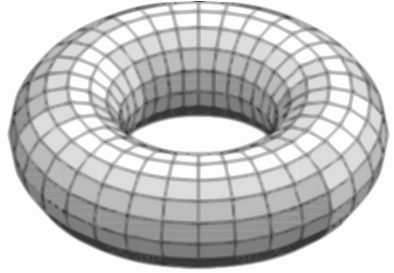
\includegraphics[scale=0.35]{pics/Torus.png}}
	\end{picture}
\end{minipage}	

\subsection{Die Idee}
Eine Idee kann viele Eigenschaften haben, die wichtigen Faktoren um andere Menschen von ihr zu überzeugen lassen sich allerdings grob durch die drei folgenden modellieren. 
Die Qualität, die Komplexität, als auch eine arbiträre durch Zahlen ermöglichte Darstellung des Raumes in dem die Idee angesiedelt ist, im folgenden Weltanschauungswert genannt, ergeben zusammen eine Idee.  \\
Die Qualität einer Idee soll den Grad ihrer Überzeugungskraft repräsentieren. Ein hoher Qualitätswert deutet auf eine qualitativ hochwertige Idee hin.
Die Komplexität hängt mit diesem Wert zusammen, ist allerdings nicht der Selbe, da auch nicht sehr überzeugende Ideen komplex und elaboriert sein können und umgekehrt. Es kann daher komplexe aber gleichzeitig qualitativ schlechte Ideen geben.

\subsection{Der Mensch}
Ein Mensch besitzt zwei für die Simulation relevante, darstellbare Eigenschaften. 
Die eine ist die Idee selbst, die andere ist ein Weltanschauungswert, ähnlich der der Idee. 
Allerdings repräsentiert der Weltanschauungswert des Menschen s restlichen Ideen, welche er besitzt, die allerdings nicht direkt das Themengebiet der untersuchten Ideen-Gruppe berühren, sondern nur indirekte Einflüsse darauf haben. 
Ein Beispiel hierfür wäre das Mathematikverständnis eines Menschen der Antike betreffend der Frage ob die Erde einer Kugel ähnelt oder nicht.

\subsection{Ablauf}
Zuerst wird eine Population von Menschen mit Ideen durchschnittlich geringer Qualität und Komplexität mit zufälligen Weltanschauungswerten in der Welt geschaffen. 
Die Weltanschauungswerte der Menschen sind in der Nähe ihrer initialen Ideen angesiedelt. \\
Nun beginnen die verschiedenen Menschen in Runden auf der Welt zu ziehen. 
Zuerst wird die Möglichkeit der Entwicklung einer neuen Idee und\/oder die Veränderung der Weltanschauungswerte evaluiert, diese ist relativ gering, tritt jedoch dem Gesetz der großen Zahlen folgend bei einigen Individuen alle paar Runden ein. 
Daraufhin werden die Möglichkeiten zur Kommunikation erfasst. Sollte ein anderes Individuum sich in Reichweite befinden, wird mit einer gewissen Wahrscheinlichkeit ein Kommunikationsversuch gestartet. 
Die Wahrscheinlichkeit resultiert aus dem menschlichen Verhalten nicht mit jedem Individuum aus seiner Umgebung Konversation zu betreiben.
zum Schluss wird ein Individuum seine Möglichkeiten zur Bewegung evaluieren.

\subsection{Entwicklung}
Die Entwicklung einer Idee erfolgt durch Mutation.
Jeder Mensch hat jede Runde eine Mutationschance sowohl für den Qualitäts-, Komplexitätskomplex, als für den Weltanschauungskomplex.
Beide Mutationen laufen ähnlich ab, zuerst wird eine Richtung gewählt, um zu gewährleisten dass die Eigenschaften nicht in 2 Richtungen mutieren. 
Darauf werden die Mutationsraten der einzelnen Elemente berechnet und diese angepasst.
Bei dem Weltanschauungskomplex existiert noch die finale Absicherung, dass die Differenz beider Werte einen nicht Schwellwert überschreiten.

\subsection{Kommunikation, Konkurrenz und Einschränkungen}
\begin{minipage}[t]{0.48\textwidth}
Bevor es zu einer Kommunikation kommt, muss ein möglicher Kommunikationspartner gefunden werden.
Dieser muss sich (wie rechts dargestellt) in einem benachbartem Feld befinden. 
So können die grüne und die blaue Idee miteinander konkurrieren, der Violetten ist dies allerdings nicht möglich. 
Sollten mehrere Kommunikationspartner zur Verfügung stehen, so werden alle betrachtet und einer wird fair ausgewählt.  \\
Die eigentliche Kommunikation ist in drei Phasen geteilt. 
Nun da ein Kommunikationspartner gefunden ist, wird entschieden ob die beiden sich austauschen.
\end{minipage}
\begin{minipage}[t]{0.48\textwidth}
\begin{picture}(0,0)
		\put(15,-165){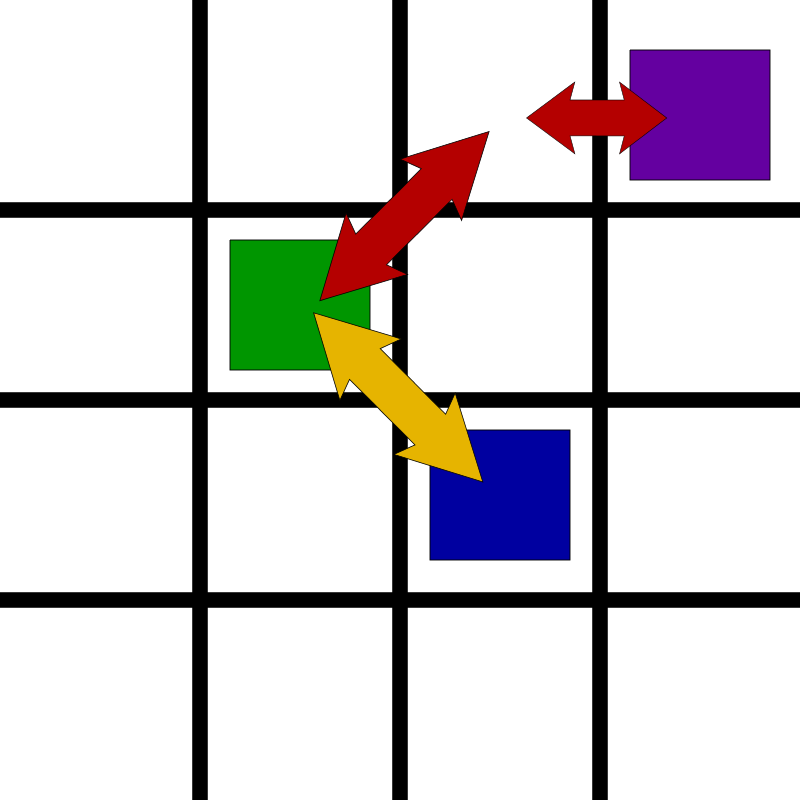
\includegraphics[scale=0.2]{pics/GridComm.png}}
		\put(25,-185){
		\begin{minipage}{0.7\textwidth}
			Kommunikationsmöglichkeiten
		\end{minipage}
		}
\end{picture}
\end{minipage}
\quad \\ \quad \\
Ist dies geschehen und positiv ausgefallen muss berechnet werden, ob sie einander überzeugen können.
Dies hängt von Faktoren wie der Komplexitätsdifferenz und den Unterschieden zwischen dem Weltanschauungswert der Zielperson und der Ursprungsidee ab. Je höher die Komplexitätsdifferenz ist, desto größer ist die Wahrscheinlichkeit, dass eine Überzeugung fehlschlägt, da davon auszugehen ist, dass die beiden Menschen auf verschiedenen Ebenen denken und sich nicht von dem anderen überzeugen lassen wollen. Die Inkompatibilität sich stark unterscheidender Weltanschauungswerte sollte auf der Hand liegen. \\
Sollte eine Kompatibilität festgestellt werden, so muss ermittelt werden, welche der beiden Ideen die andere dominiert. Dies geschieht anhand eines Qualitätsabgleichs mit einem zufälligen temporären Aufschlag auf die Qualitätswerte beider Ideen. Dieser Aufschlag repräsentiert mögliche sonstige Einflüsse wie beispielsweise die Eloquenz des Gegenübers. \\
Wenn nun ein Gewinner feststeht, muss der Verlierer seine Meinung, respektive seine Idee ändern. Dies ist leicht durch die direkte Übernahme zu garantieren. Allerdings muss auch der Weltanschauungswert des verlierenden Menschens an die Idee angepasst werden, da die Idee einen Einfluss auf diesen hat. \\

\subsection{Bewegung}
Nicht alle Menschen gehen einer missionarischen Tätigkeit (welche Anschauung sie auch immer vertreten) sondern vielen anderen Beschäftigungen nach und verbreiten ihre Ideen eher ungerichtet an andere. \\
Nun gäbe es die Möglichkeit diese Tätigkeiten zu simulieren, dies erscheint allerdings in Anbetracht der Projekt-Idee wenig zielführend, daher ist die Wahl der Bewegungsart auf eine zufällige Wahl aus den maximal 9 erreichbaren Feldern gefallen, welche als eine ausreichende Abstraktion der anderen Tätigkeiten erscheint. 
Natürlich existieren auch Missionare in dem Sinn, dass sie ihre Idee einer breiten Masse zugänglich machen, allerdings muss ein zu überzeugender Mensch erst einmal (zum Beispiel durch Mundpropaganda oder zufällige Entdeckung, wenn der Missionar noch unbekannt ist) auf diese Missionare stoßen.
Somit stellt dies kein Argument für die Einschränkung einer zufälligen Bewegung dar. \\ \\
\begin{minipage}[t]{0.38\textwidth}
Die möglichen Bewegungen sind hier noch einmal grafisch in rot zu sehen dargestellt (die Möglichkeit still zu stehen bleibt bestehen, obwohl nicht markiert). \\
\end{minipage}
\begin{minipage}[t]{0.58\textwidth}
\begin{picture}(0,0)
		\put(30,-120){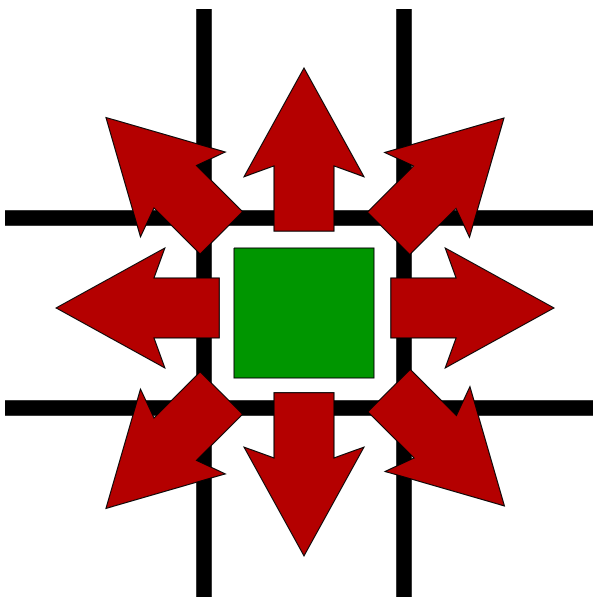
\includegraphics[scale=0.3]{pics/GridMov.png}}
\end{picture}
\end{minipage}


\section{Implementation}
\subsection{Logik und Idee \& Mensch}
Die im Abschnitt Modellierung geschilderten Modellierungen sind eins zu eins in Software umgesetzt, mit der Ausnahme, dass ein Mensch/ eine Idee durch einen struct mit 4 Feldern repräsentiert wird.

\section{Probleme}
%TODO content

%TODO bibliography with used mats
\pagebreak
%\nocite{*}
